%%
%% ****** ljmsamp.tex 13.06.2018 ******
%%
\documentclass[
11pt,%
tightenlines,%
twoside,%
onecolumn,%
nofloats,%
nobibnotes,%
nofootinbib,%
superscriptaddress,%
noshowpacs,%
centertags]%
{revtex4}
\usepackage{ljm}
\usepackage{listings}
\usepackage{xcolor}

\usepackage[utf8]{inputenc}
\usepackage[russian]{babel}

\lstset{
language=C++,
basewidth=0.5em,
xleftmargin=45pt,
xrightmargin=45pt,
basicstyle=\small\ttfamily,
%keywordstyle=\bfseries\underbar,
keywordstyle=\color[rgb]{0,0,1},
numbers=left,
numberstyle=\tiny,
stepnumber=1,
numbersep=10pt,
showspaces=false,
showstringspaces=false,
showtabs=false,
frame=trBL,
tabsize=2,
captionpos=t,
breaklines=true,
breakatwhitespace=false,
escapeinside={\%*}{*)}
}

\begin{document}

\titlerunning{Vectorization} % for running heads
\authorrunning{Rybakov} % for running heads
%\authorrunning{First-Author, Second-Author} % for running heads

\title{Векторизация целочисленного программного контекста \\ в задаче декомпозиции графа}
% Splitting into lines is performed by the command \\
% The title is written in accordance with the rules of capitalization.

\author{\firstname{А.~А.}~\surname{Рыбаков}}
\email[E-mail: ]{rybakov_aa@nrcki.ru,rybakov@jscc.ru,rybakov.aax@gmail.com}
\affiliation{Национальный исследовательский центр «Курчатовский институт», 123182, Москва, пл. Академика Курчатова, д. 1, Россия.}

%\author{\firstname{B.}~\surname{Second-Author}}
%\email[E-mail: ]{Second.Author@email.com}
%\affiliation{Place of work and/or the address of the first and second authors}
%\affiliation{Place of work and/or the address of second authors}
%\noaffiliation % If the author does not specify a place of work.

\firstcollaboration{(Submitted by TODO)} % Add if you know submitter.
%\lastcollaboration{ }

%\received{June 13, 2018} % The date of receipt to the editor, i.e. December 06, 2017

\begin{abstract} % You shouldn't use formulas and citations in the abstract.
Статья посвящена проблеме векторизации программного контекста, преимущественно работающего с целыми числами и содержащего большое количество операций передачи управления.
Такой программный контекст зачастую встречается в задачах комбинаторной оптимизации, в которых приходится работать с дискретными структурами данных, косвенностью при обращении в память и гнездами циклов с нерегулярным числом итераций.
Эти факторы негативно влияют на применение векторизации, а автоматическая векторизация для такого контекста практически невозможна.
В статье рассматривается возможность использования набора инструкций AVX-512 для векторизации кода с перечисленными особенностями, так как преимущества маскированных векторных операций позволяют достичь ускорения даже при наличии таких узких мест.
Применение векторизации рассматривается на примере алгоритма пузырькового роста декомпозиции графа, где граф представлен в виде списков смежности вершин.
Для рассматриваемого алгоритма описан метод применения векторизации к гнездам циклов с использованием целочисленных маскированных векторных инструкций из набора AVX-512F.
Векторизованный алгоритм декомпозиции апробирован на графах с количеством вершин до 4 миллионов.
Проведены практические эксперименты на микропроцессоре Intel Xeon Phi 7290 Knights Landing, которые показали ускорение программного кода в диапазоне 1,7 -- 2,2 раз в зависимости от размера расчетной сетки.
\end{abstract}

\subclass{68W10, 68R10} % Enter 2010 Mathematics Subject Classification.

\keywords{векторизация, AVX-512, целочисленный программный контекст, комбинаторная оптимизация, декомпозиция графа, алгоритм пузырькового роста} % Include keywords separeted by comma.

\maketitle

% Text of article starts here.

\section{Introduction}

Высокопроизводительные вычисления позволяют производить моделирование природных и технологических процессов с высокой степенью детализации, одновременно учитывать множество факторов различного происхождения, быстро анализировать многочисленные варианты.
Это позволяет получать картину исследуемого процесса с требуемой точностью, максимально отражая реально существующую ситуацию взамен дорогостоящих, опасных или просто невозможных натурных экспериментов.
Использование суперкомпьютерных технологий позволяет существенно снизить стоимость и сроки создания новых конкурентоспособных изделий, объектов и систем.
Спектр областей применения высокопроизводительных вычислений очень широк.
Так, с помощью суперкомпьютерного моделирования решаются задачи газовой и гидродинамики \cite{01Smirnov}, молекулярной динамики \cite{02Guo}, физики плазмы \cite{03Asch}, механики твердого тела \cite{04Morgan}, математики \cite{05Lohiya} и другие.
Высокопроизводительные вычисления применяются для решения таких больших расчетных научно-технических задач, как моделирование атмосферы \cite{06Kang}, проектирование летательных аппаратов \cite{07Morad}, исследование нефтяных и газовых месторождений \cite{08Eremin}, моделирование крупных молекул и многоатомных систем \cite{09Yan} и многих других.

При решении расчетной задачи на вычислительном кластере необходимо выполнять распараллеливание между его узлами для ускорения вычислений \cite{10Voevodin}.
Следующий уровень распараллеливания вычислений -- распараллеливание в рамках одного вычислительного узла на общей памяти \cite{11Zhou}.
Самым низким уровнем распараллеливания вычислений можно считать векторизацию – распараллеливание на уровне отдельных инструкций \cite{12Feng}.

Векторизация является важной низкоуровневой оптимизацией программного кода, с помощью которой можно достичь кратного ускорения суперкомпьютерных приложений.
Все основные современные микропроцессорные архитектуры (x86, ARM, Power, <<Эльбрус>>, LoongArch, Sunway и другие) поддерживают векторные вычисления, причем наблюдается тенденция на увеличение размера вектора (на сегодняшний день максимальная длина равна 512 битам, но уже сейчас логически эта длина не ограничена, учитывая наборы векторных инструкций с переменной длиной
вектора).

Сейчас наиболее перспективным набором векторных инструкций является набор AVX-512, так как в нем поддержана возможность выборочной обработки элементов векторов с помощью векторных масок.
Эта уникальная возможность позволяет векторизовать сложный программный контекст, содержащий команды передачи управления, гнезда циклов и вызовы функций.
Можно считать, что впервые набор векторных инструкций AVX-512 был поддержан в 2016 году в микропроцессорах Intel Xeon Phi Knights Landing (KNL), так как более раннее поколение Intel Xeon Phi Knights Corner (KNC) представляет собой ускоритель, и векторный код для него не является x86 совместимым.
С этого момента вопросы векторизации приложений активно обсуждаются в научном сообществе.
Можно отметить множество работ по векторизации программного контеста в приложении к различным предметным областям: газодинамические решатели \cite{12-1Kulikov}, инструменты шифрования \cite{12-2Buhrow}, анализ временных рядов \cite{12-3Quislant}, сортировка массива чисел \cite{12-4Blacher}, быстрое преобразование Фурье \cite{12-5Sansone} и многое другое.

В этой работе будем рассматривать применение векторизации с помощью набора инструкций AVX-512 к целочисленному программному контексту, содержащему циклы с нерегулярным количеством итераций.
В качестве такого контеста возьмем алгоритм пузырькового роста декомпозиции графа, в котором выполняется одновременный обход графа в ширину от случайным образом расположенных инициирующих вершин.

\section{Алгоритм пузырькового роста декомпозиции графа}

В настоящее время существует большое разнообразие алгоритмов декомпозиции графов, которые применяются в зависимости от размера обрабатываемого графа и требований, предъявляемых к качеству декомпозиции \cite{13Ayall}.
При этом требования к размеру обрабатываемых графов постоянно увеличиваются, и сегодня задача декомпозиции рассматривается для графов, содержащих десятки миллионов ячеек и более \cite{14Lee}.
При выполнении обработки графов основной операцией является получение по заданной вершине инцидентных ей ребер и соседних с ней вершин.
Способ выполнения этого действия зависит от внутреннего представления графа в памяти компьютера \cite{15Ahmed,16Salwasser}.
Будем рассматривать такое представление неориентированного графа, в котором для каждого индекса вершины доступен список соседних с ней вершин.
Рассмотрим следующий алгоритм декомпозиции графа -- алгоритм пузырькового роста -- являющийся одним из наиболее простых с точки зрения логики работы.

\begin{figure}[h]
\setcaptionmargin{5mm}
%\onelinecaptionsfalse % if the caption is multiline
\onelinecaptionstrue  % if the caption is one-line
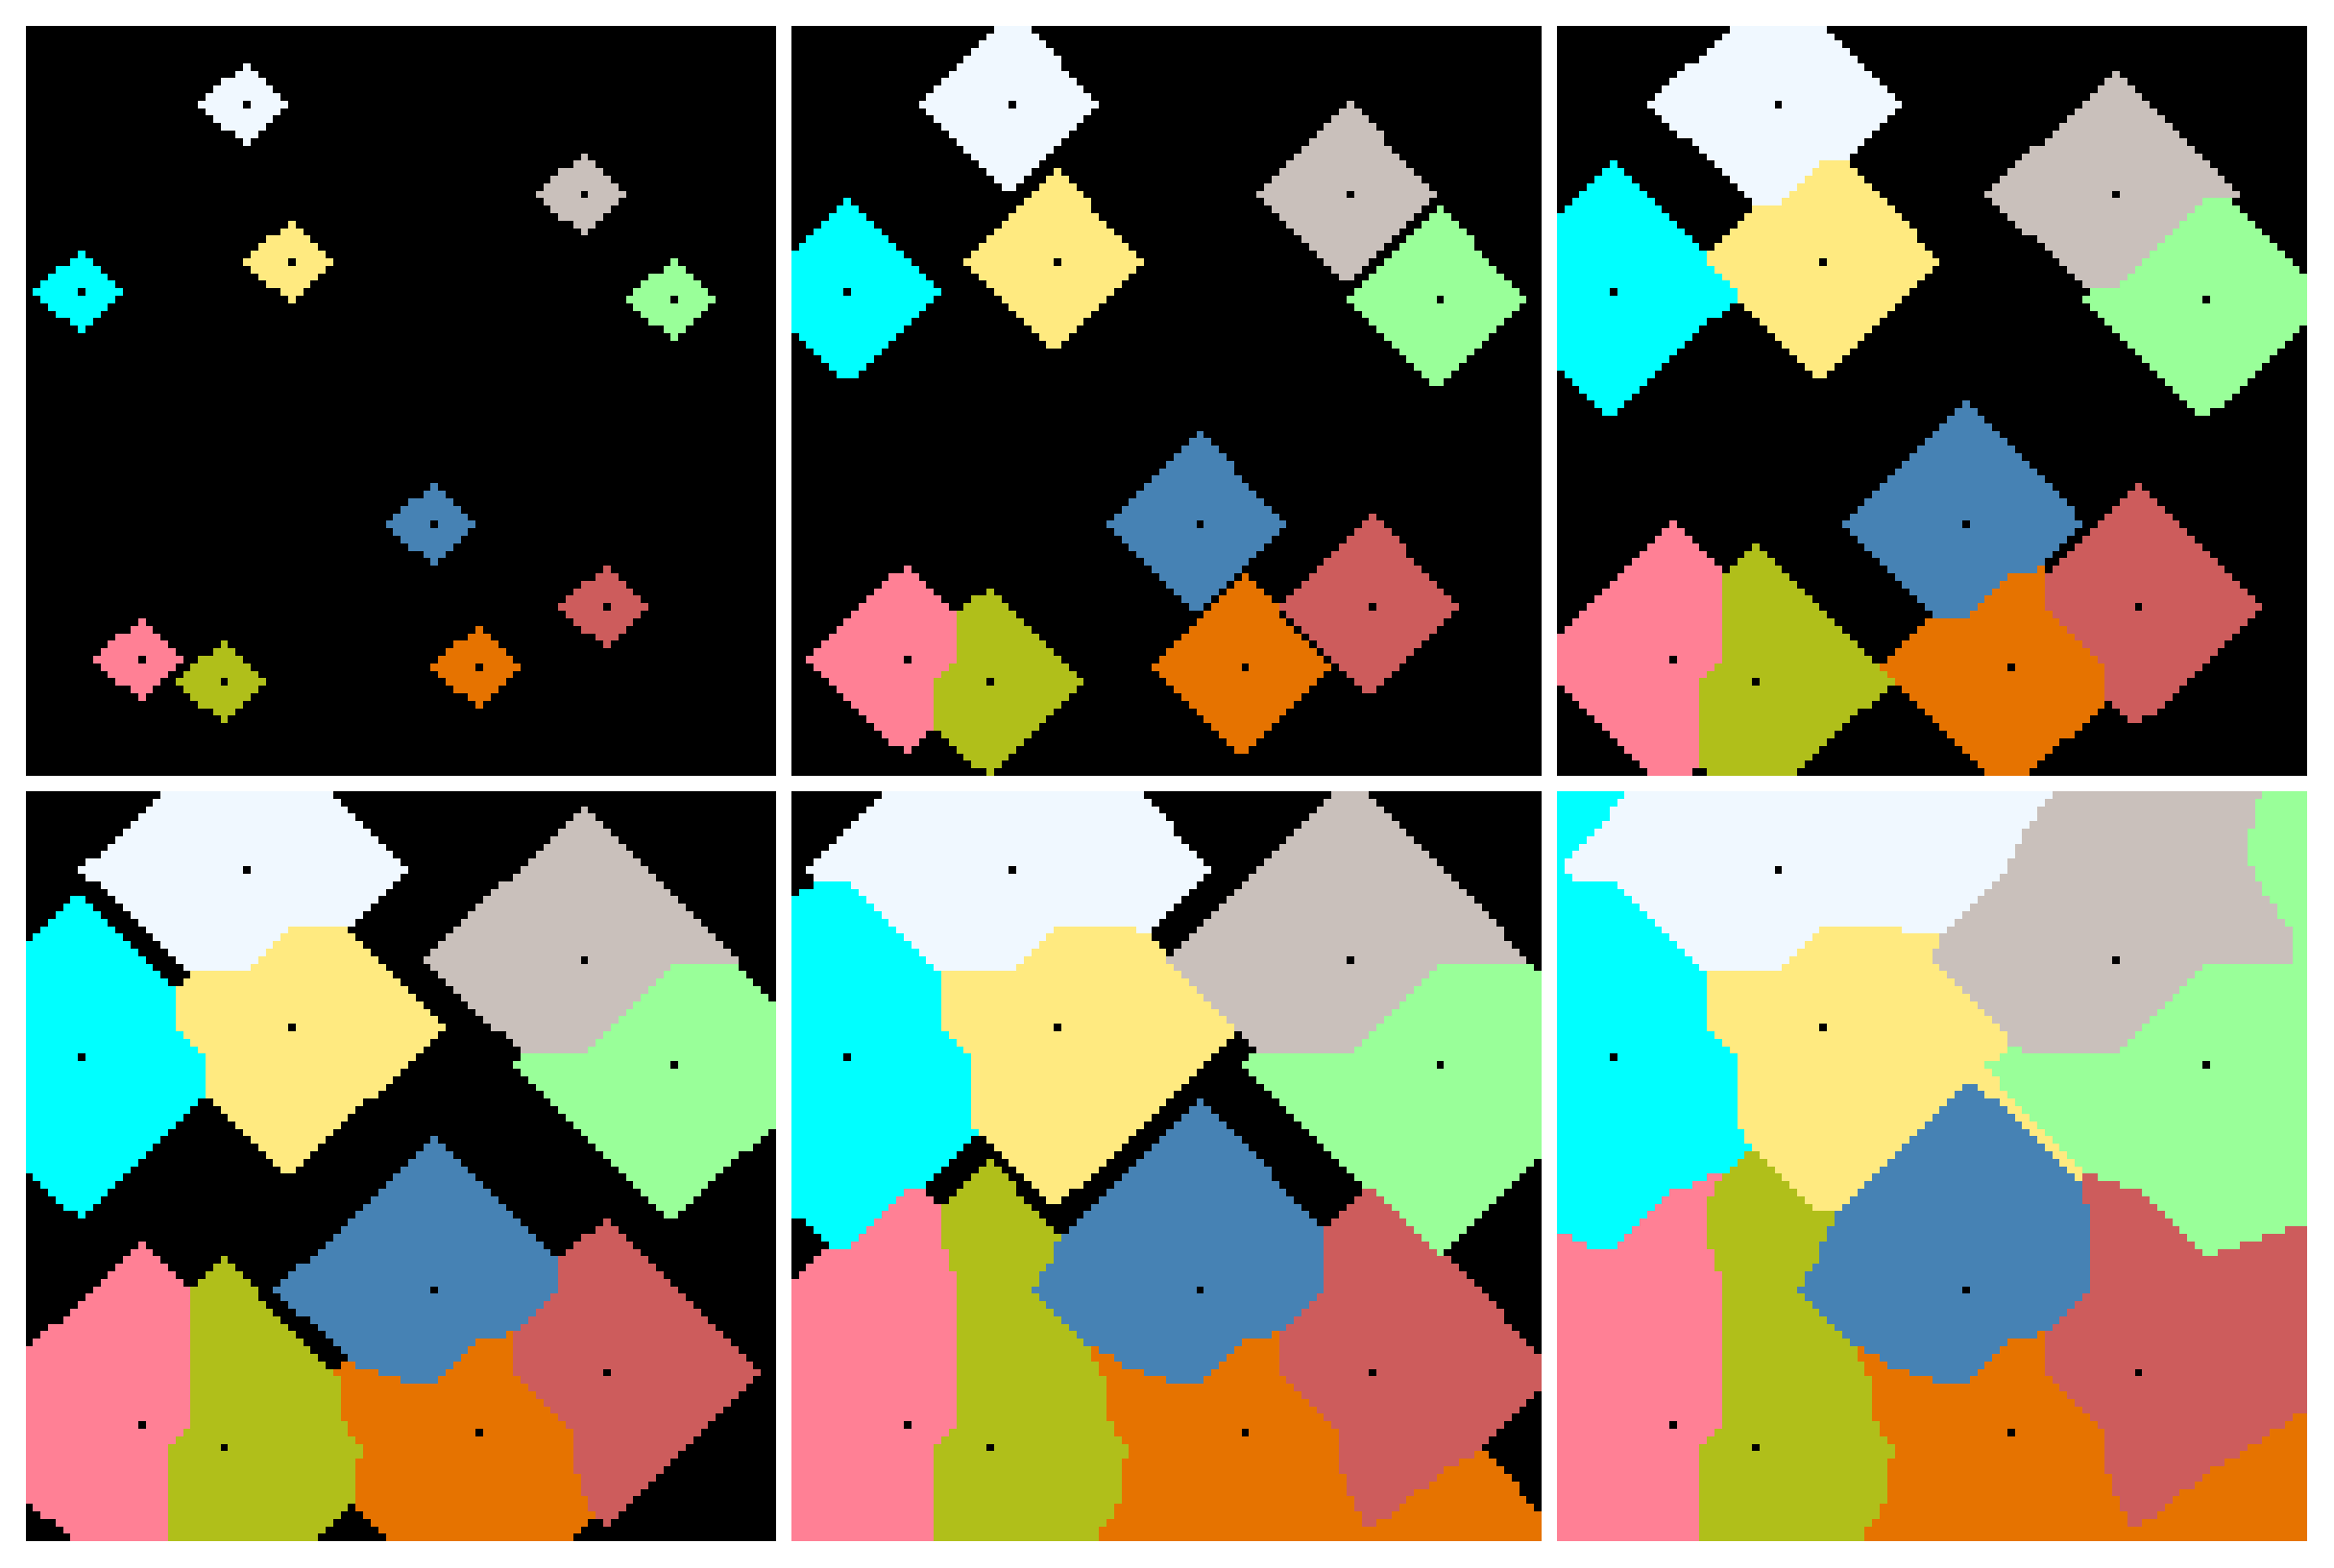
\includegraphics[width=0.65\textwidth]{pics/incr.pdf}
\captionstyle{normal}\caption{Нарастание доменов при работе пузырькового алгоритма декомпозиции.}\label{fig:incr}
\end{figure}

Алгоритм пузырькового роста декомпозиции графа \cite{17Fan} основан на обходе графа в ширину, выполняемом одновременно, начиная с нескольких вершин.
В начале работы алгоритма случайным образом выбираются инициирующие вершины (по требуемому количеству доменов).
Каждая из выбранных вершин относится к соответствующему домену.
После этого начинается процесс одновременного наращивания доменов, при котором на каждой итерации алгоритма к каждому домену добавляется одна соседняя еще не раскрашенная вершина (при условии, что это можно сделать).
Процесс завершается, когда все вершины графа оказываются распределенными по доменам.
На рис.~\ref{fig:incr} проиллюстрирован процесс наращивания доменов от случайно выбранных вершин для графа на плоскости.

После распределения всех вершин по доменам для каждого домена вычисляется его центр, после чего центры доменов принимаются за новые инициирующие вершины, раскраска графа сбрасывается, а далее выполняется наращивание доменов от этих новых инициирующих вершин.
Этот процесс может продолжаться либо фиксированное количество раз, либо до момента достижения определенного условия (стабилизация инициирующих вершин, достижение сбалансированного разбиения, повторение ранее полученной конфигурации) \cite{18Golovchenko}.
Алгоритм пузырькового роста не гарантирует получение сбалансированного разбиения на домены или формирование коротких границ между доменами.
Однако этот алгоритм отличается своей простотой, что позволяет использовать его в качестве базовой операции в комплексных подходах к декомпозиции \cite{19Wu}.

Отметим кратко потенциал использования алгоритма пузырькового роста в семействе генетических алгоритмов \cite{20Katosh}.
Генетические алгоритмы являются природоподобными эвристическими алгоритмами, которые активно применяются для решения оптимизационных задач с большим количеством параметров \cite{21Wirayanti}.
Во время работы генетического алгоритма моделируется процесс выживания популяции, состоящей из отдельных особей, каждая из которых представляет собой решение некоторой оптимизационной задачи.
Для реализации алгоритма должно быть определено понятие генотипа (некоторого кода особи), реализован процесс создания особи по его генотипу, определена функция пригодности особи, а также реализованы операции скрещивания и мутации особей на уровне генотипов.
В процессе развития популяции наиболее слабые особи вымирают, а более приспособленные оставляют потомство, что приводит к повышению среднего значения функции пригодности особей в популяции.
Генетические алгоритмы применимы для решения задач комбинаторной оптимизации, в частности для задачи декомпозиции графа.
Однако зачастую при использовании генетического алгоритма для решения задачи декомпозиции графа происходит смешивание понятия генотипа и особи.
Например, в работе \cite{22Chaouche} при декомпозиции графа в генотипе кодируется каждое ребро, а в работе \cite{23Li} в генотипе кодируется явное распределение вершин по доменам.
То есть генотип практически подменяет собой понятие особи, что приводит к существенному замедлению работы генетического алгоритма и невозможности его применения для декомпозиции больших графов.
Также применение механизмов скрещивания и мутаций непосредственно к особям вызывает сомнение с точки зрения корректности.
Простота и скорость работы алгоритма пузырькового роста позволяет использовать его в генетических алгоритмах в качестве операции построения особи из генотипа, представленного набором инициирующих вершин.
При этом в роли мутации генотипа может рассматриваться смещение инициирующей вершины к случайному соседу.
Такой подход применения алгоритма пузырькового роста внутри генетического алгоритма был апробирован на практике, и решение доступно в открытом репозитории https://github.com/r-aax/mendel.

\section{Векторизация алгоритма пузырькового роста}

Использование алгоритма пузырькового роста в качестве отдельной операции в комплексных подходах к декомпозиции графов предъявляет повышенные требования к его быстродействию.
Рассмотрим возможности по ускорению этого алгоритма с помощью векторизации.
Пусть мы имеем граф, информация о его ребрах записана в структуре \texttt{vector$<$vector$<$int$>>$ inc}, где \texttt{inc[i]} -- список номеров всех вершин, смежных с вершиной \texttt{i}.
Номера доменов, к которым относятся конкретные вершины хранятся в структуре \texttt{vector$<$int$>$ domains}.
Структура \texttt{vector$<$queue$<$int$>>$ q} -- список очередей вершин, ожидающих попадания в домены, в начале работы алгоритма очередь \texttt{q[i]} содержит только одну инициирующую вершину \texttt{i}-го домена.
Пусть требуется выполнить декомпозицию (или раскраску) на \texttt{domains\_count} доменов.
Тогда реализация алгоритма пузырькового роста доменов от инициирующих вершин может иметь следующий вид (см. листинг~\ref{lst:impl}):

\begin{lstlisting}[caption={Реализация алгоритма пузырькового роста доменов.},label={lst:impl}]
while (is_q)
{
    is_q = false;

    for (size_t c = 0; c < domains_count; ++c)
    {
        if (q[c].empty()) continue;

        is_q = true;
        n = q[c].front();
        q[c].pop();

        if (domains[n] == -1)
        {
            domains[n] = c;
            for (auto ngh : inc[n]) q[c].push(ngh);
        }
    }
}
\end{lstlisting}

Реализация алгоритма представляет собой гнездо из 3 циклов.
Внешний цикл выполняется до тех пор, пока найдется хотя бы одна непустая очередь домена (то есть остались нераспределенные по доменам вершины).
Средний цикл выполнятся по номерам доменов.
Для каждого домена берется первая необработанная вершина из соответствующей очереди, и если она еще не отнесена ни к одному домену, то она заносится в текущий домен, а все ее соседи отправляются в очередь.
Внутренний цикл -- цикл по всем соседям только что обработанной вершины, которые должны быть занесены в очередь.
Будем выполнять векторизацию представленного кода по среднему циклу, и для простоты анализа приведем реализацию для фиксированного значения \texttt{domains\_count = 16} (это позволит избавиться от среднего цикла, и заменить его набором отдельных векторных операций).

Для выполнения векторизации вначале необходимо избавиться от STL структур vector и queue, так как они имеют свою внутреннюю реализацию, и векторизация операций по работе с ними невозможна.
Вместо структуры \texttt{vector$<$int$>$} будем хранить информацию о списке соседних вершин просто в массиве, 0-м элементом которого будет его размер.
Очередь queue также будет имитировать с помощью массива и индексов \texttt{front} и \texttt{back}, указывающих на первый и последний элементы очереди соответственно.
Тогда операция \texttt{push(v)} будет соответствовать записи в массив по индексу \texttt{back} с его продвижением, а операция \texttt{pop} будет соответствовать просто продвижению индекса \texttt{front}.
Очередь пуста если ее индекс \texttt{front} больше индекса \texttt{back}.

\begin{figure}[h]
\setcaptionmargin{5mm}
\onelinecaptionsfalse % if the caption is multiline
%\onelinecaptionstrue  % if the caption is one-line
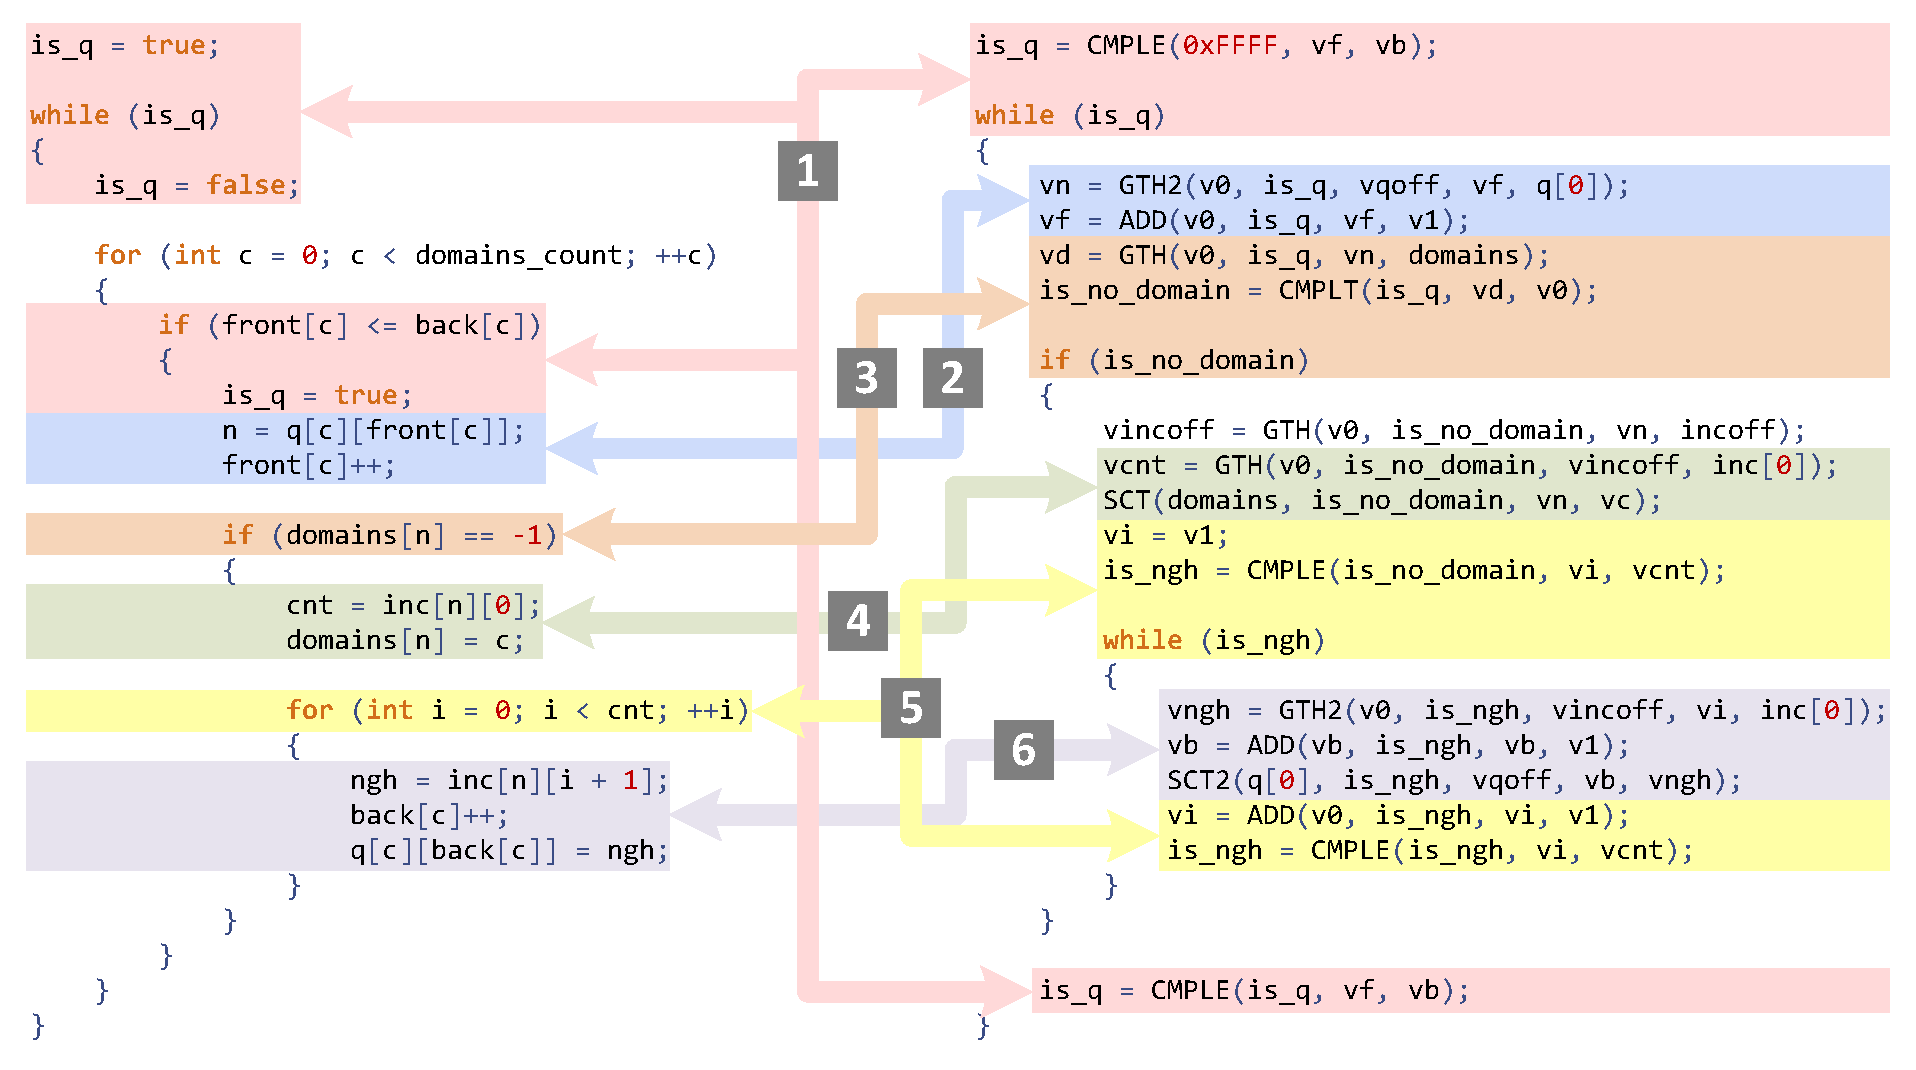
\includegraphics[width=0.85\textwidth]{pics/code.pdf}
\captionstyle{normal}\caption{Векторизация программного кода алгоритма пузырькового роста путем замены скалярных инструкций на векторные аналоги.}\label{fig:code}
\end{figure}

На рис.~\ref{fig:code} представлены скалярная и векторная версии программного кода реализации алгоритма пузырькового роста.
В векторной версии через \texttt{ADD}, \texttt{GTH}, \texttt{SCT} обозначаются функции-интринсики \texttt{\_mm512\_mask\_add\_epi32}, \texttt{\_mm512\_mask\_i32gather\_epi32}, \texttt{\_mm512\_i32scatter\_epi32} соответственно (\texttt{GTH2} и \texttt{SCT2} это те же операции \texttt{GTH} и \texttt{SCT}, только использующие сразу два смещения от базового адреса).
Через \texttt{CMPLE}, \texttt{CMPLT} обозначены вызовы функции-интринсика \texttt{\_mm512\_mask\_cmp\_epi32\_mask} с параметрами сравнения \texttt{\_MM\_CMPINT\_LE} и \texttt{\_MM\_CMPINT\_LT} соответственно.
На рис.~\ref{fig:code} цифрой <<1>> обозначена векторизация условия продолжения выполнения внешнего цикла (цикл завершает работу, если все очереди доменов пусты).
Цифрой <<2>> обозначена векторизация извлечения следующей вершины из каждой очереди.
Цифрой <<3>> обозначена проверка принадлежности извлеченных вершин к какому-либо домену (в векторной версии формируется маска \texttt{is\_no\_domain} -- маска с номерами доменов, в которые добавляется новая вершина).
Цифрой <<4>> обозначена векторизация помещения рассматриваемой вершины в текущий домен и получение количества ее соседей.
Цифра <<5>> -- обработка всех соседей только что помещенной в домен вершины, и цифра <<6>> -- добавление этих соседей в соответствующие очереди.

Стоит отметить, что векторизованная версия представленного алгоритма не является полностью эквивалентной скалярной версии.
Вполне может оказаться, что на какой-то итерации внешнего цикла из двух или более разных очередей одновременно будет извлечена одна и та же вершина.
В этом случае в векторной версии она будет отнесена к домену с наибольшим номером (хотя в скалярном аналоге, она бы попала в домен с меньшим номером).
Это несоответствие можно устранить путем разворачивания векторов \texttt{vn} и \texttt{vc} при записи в массив \texttt{domains} (цифра <<4>> на рис.~\ref{fig:code}), но это не делалось, чтобы не усложнять код.

\begin{figure}[h]
\setcaptionmargin{5mm}
\onelinecaptionsfalse % if the caption is multiline
%\onelinecaptionstrue  % if the caption is one-line
\begin{tabular}{ll}
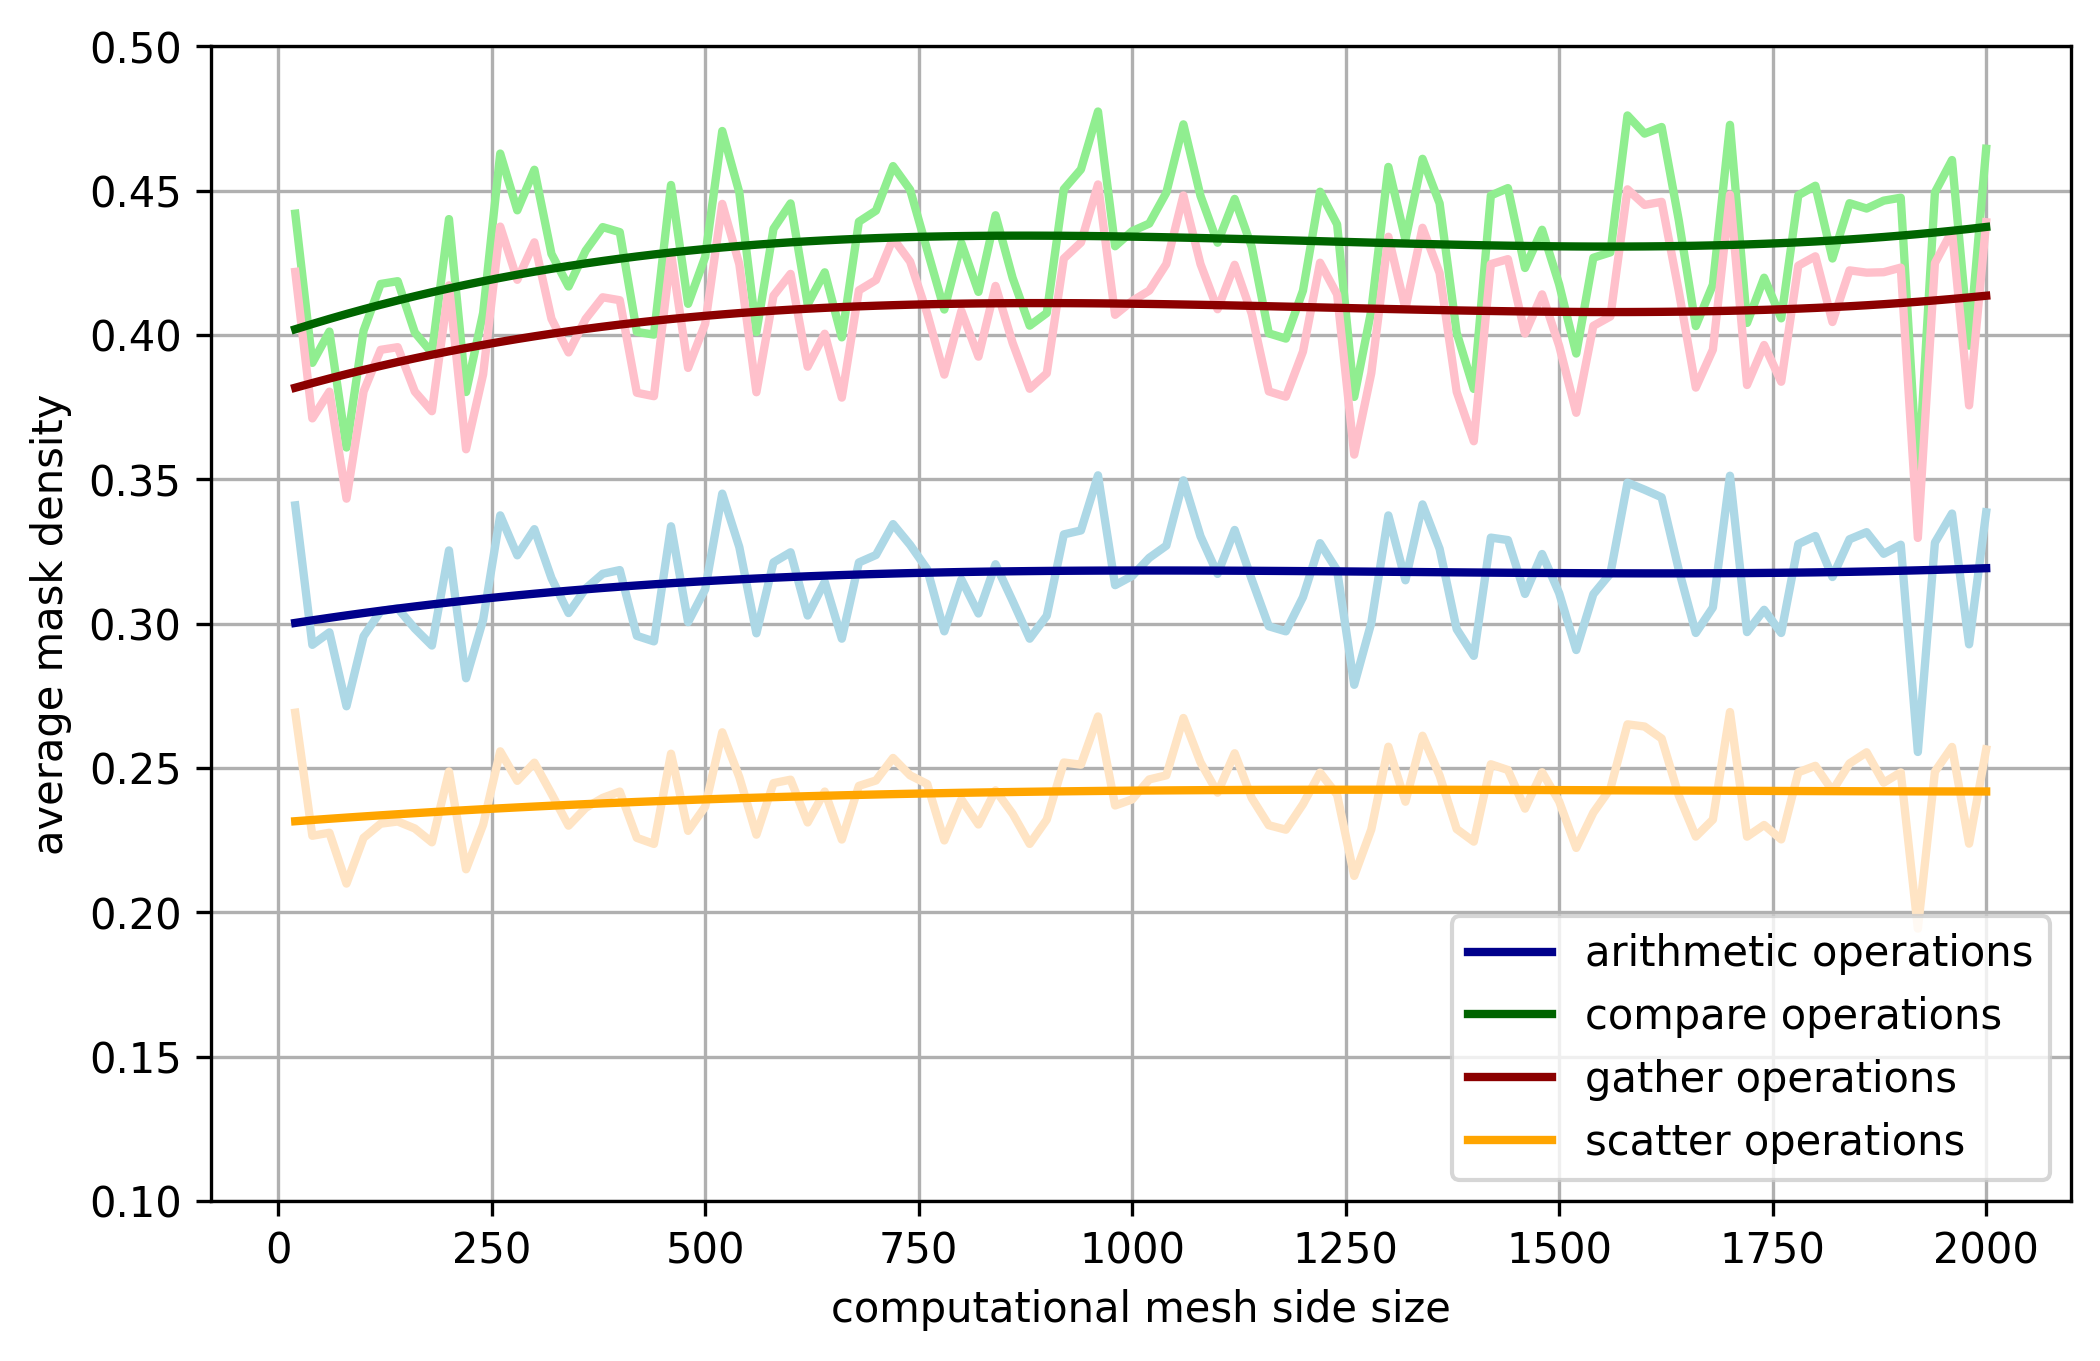
\includegraphics[width=0.45\textwidth]{pics/chart_statistics_eng.png}
&
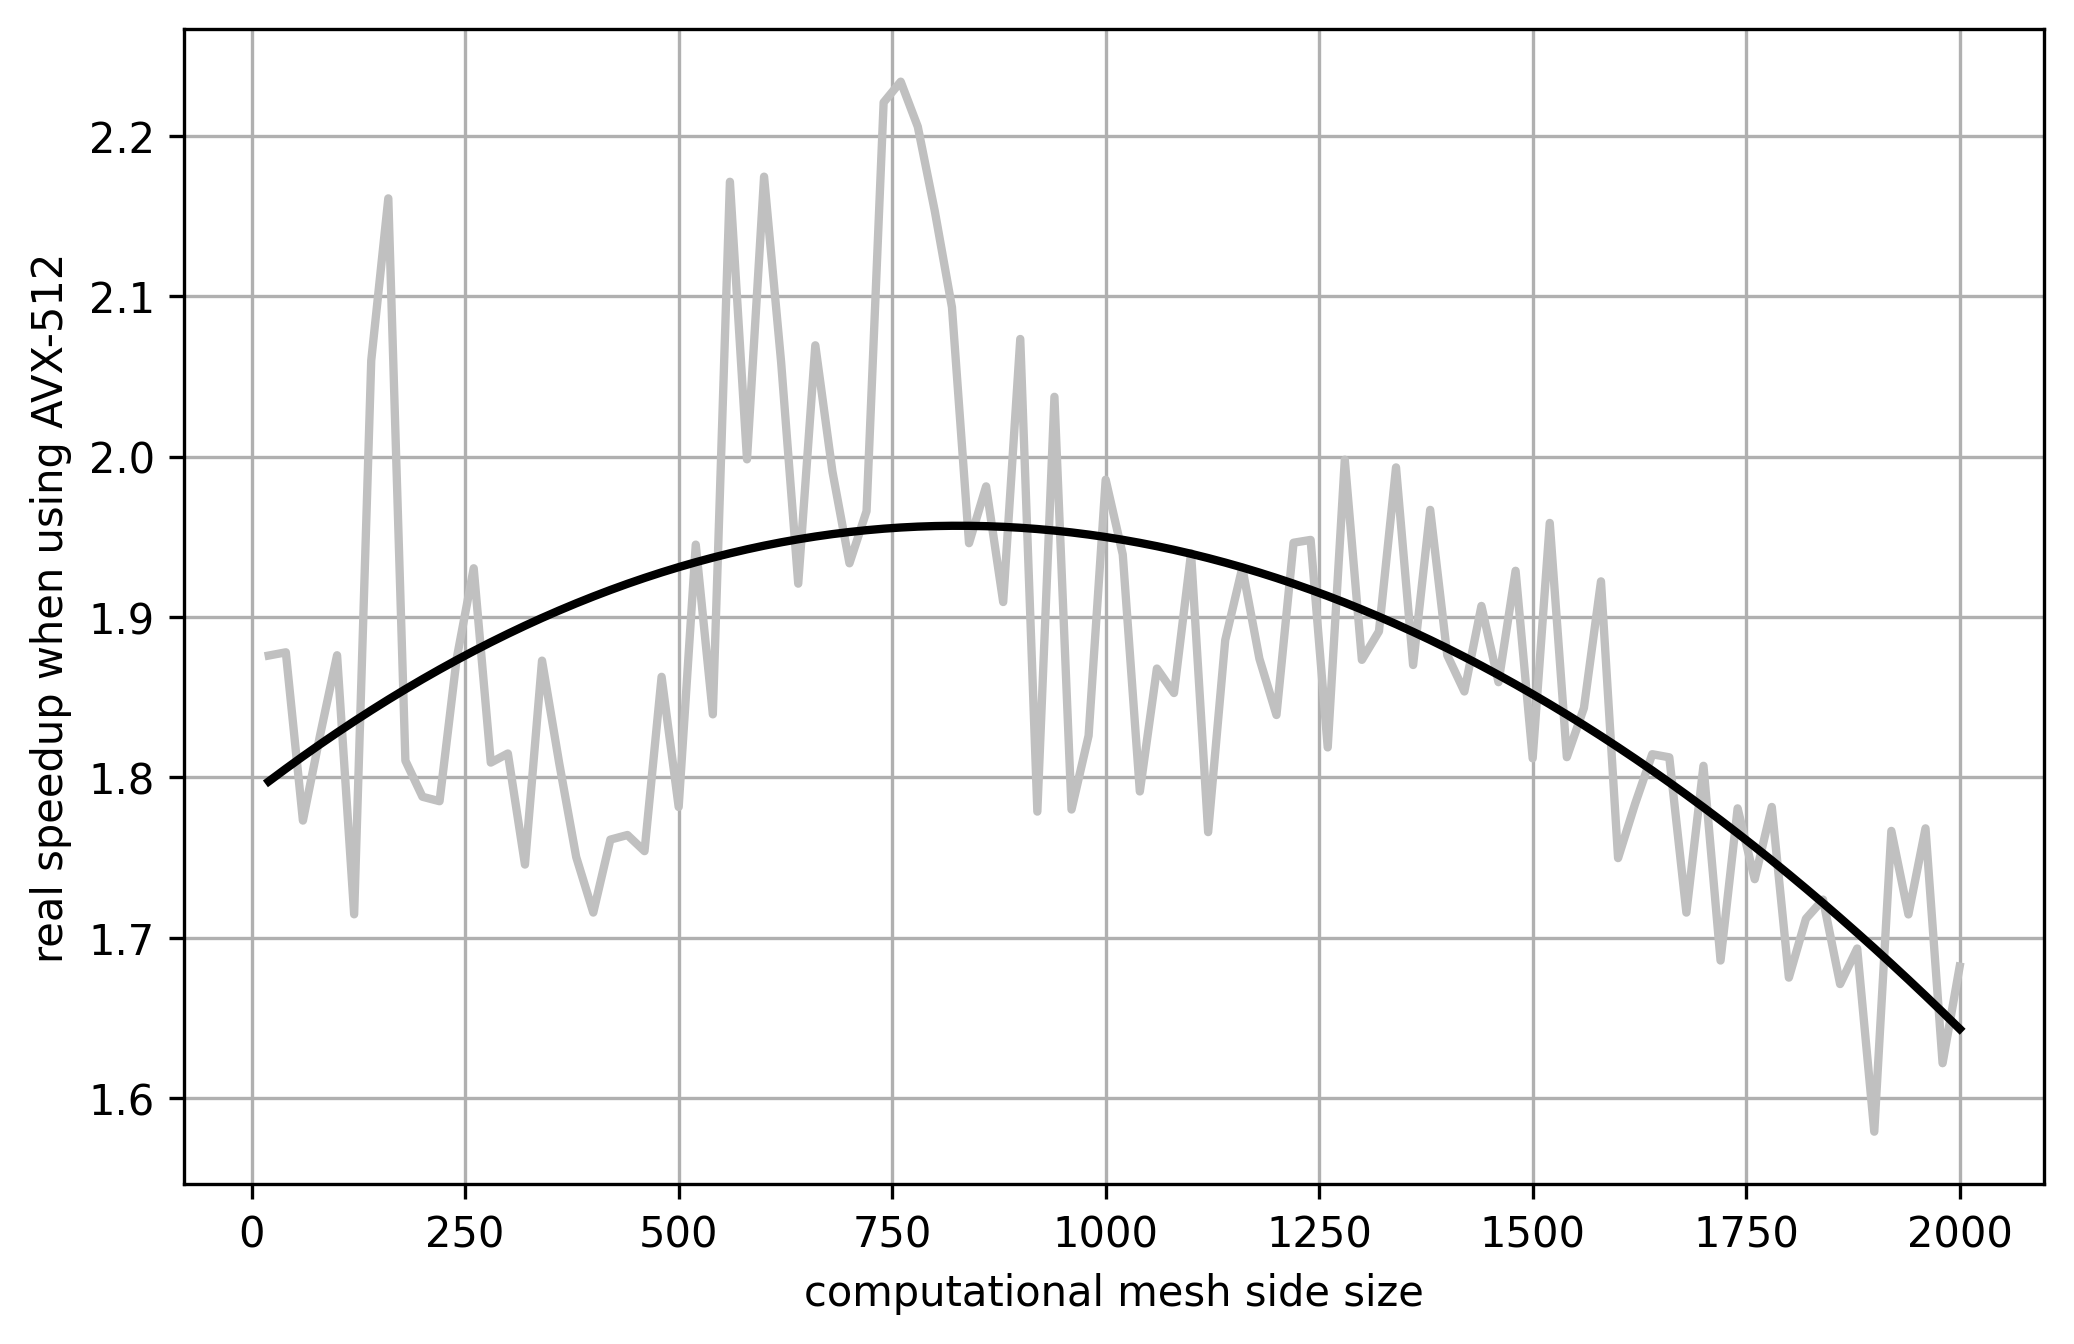
\includegraphics[width=0.45\textwidth]{pics/chart_speedup_eng.png}
\end{tabular}
\captionstyle{normal}\caption{Средняя плотность масок операций AVX-512 разных классов (слева) и ускорение вычислений, полученное на Intel Xeon Phi 7290 Knights Landing (справа).}\label{fig:chart}
\end{figure}

Для оценки эффективности проведенной векторизации были произведены запуски на дуальных графах поверхностных прямоугольных расчетных сеток со стороной от 20 до 2000 ячеек (то есть на графах с количеством вершин от 400 до 4 млн).
На рис.~\ref{fig:chart} слева представлена собранная статистика плотности масок (доля выставленных битов) векторных операций различных типов.
Из этих графиков можно сразу сделать вывод о невысокой эффективности векторизации, так как плотность масок арифметических операций и операций записи в память оказались довольно низкими (примерно 0,3 и 0,25 соответственно).

Замеры реального ускорения выполнялись для тех же графов на микропроцессоре Intel Xeon Phi 7290 Knights Landing, результаты представлены на рис.~\ref{fig:chart} справа, для удобства приведен также график сглаженного показателя ускорения.
Анализирую график сглаженного показателя ускорения, можно отметить, что максимум наблюдается при размере стороны расчетной сетки в районе 750 и равен примерно 1,95.
Снижение ускорения при уменьшении стороны расчетной сетки связано с увеличение количества конфликтов при обработке следующих вершин из очередей доменов.
Снижение ускорения при увеличении стороны расчетной сетки связано с увеличением разброса смещений при выполнении операций gather/scatter, что приводит к промахам в кэш-память.

\section{Conclusion}

В статье был рассмотрен алгоритм пузырькового роста, используемый для декомпозиции графа.
Этот алгоритм применяется для выполнения декомпозиции как в роли самостоятельного метода, так и в составе других, более комплексных подходов к декомпозиции.
Была рассмотрена реализация, в которой для каждого домена поддерживается своя очередь обрабатываемых вершин графа.
Такой подход допускает одновременную обработку очередей доменов, что делает возможным применение векторизации для ускорения вычислений.
Был предложен вариант векторизации алгоритма по среднему циклу гнезда для фиксированного количества доменов, равного 16.
Для полученного варианта векторизации была собрана статистика плотности векторных масок векторных операций в результирующем коде, которая показала крайне низкие значения для арифметических операций (около 0,3) и операций записи в память (около 0,25).
Такая низкая плотность масок связана с поведением внутреннего цикла, количество итераций которого можно охарактеризовать как нерегулярное, то есть никак не зависящее от номера итерации среднего цикла.
Замеры ускорения на микропроцессоре Intel Xeon Phi 7290 Knights Landing продемонстрировали ускорение в диапазоне 1,7-2,2 раза для рассматриваемых графов с количеством ячеек от 400 до 4 млн.
Такие невысокие результаты ускорения объясняются прежде всего нерегулярным количеством итераций циклов в гнезде, а также обилием операций множественного обращения в память gather/scatter.

\begin{acknowledgments}
Работа выполнена в рамках государственного задания НИЦ «Курчатовский институт».
\end{acknowledgments}

%
% The Bibliography
%

\begin{thebibliography}{99}

\bibitem{01Smirnov}
\refitem{article}
E.~M.~Smirnov, D.~K.~Zaitsev, A.~A.~Smirnovsky et al., \textquotedblleft Assessment of several advanced numerical algorithms implemented in the CFD code SINF/Flag-S for supercomputer simulations, \textquotedblright Supercomputing Frontiers and Innovations \textbf{11} (2), 14--31 (2024). https://doi.org/10.14529/jsfi240202

\bibitem{02Guo}
\refitem{article}
Z.~Guo, D.~Lu, Y.~Yan et al., \textquotedblleft Extending the limit of molecular dynamics with ab initio accuracy to 10 billion atoms, \textquotedblright 27th ACM SIGPLAN Symposium on Principles and Practice of Parallel Programming, April 2--6, Seoul, Republic of Korea (2022). https://doi.org/10.1145/3503221.3508425

\bibitem{03Asch}
\refitem{article}
C.~Asch, E.~Francesquini, and E.~Meneses, \textquotedblleft An implementation of a plasma physiscs application for distributed-memory supercomputers using a directive-based programming framework, \textquotedblright Revista Colombiana de Computaci\'on \textbf{25} (1), 39--47 (2024). https://doi.org/10.29375/25392115.5053

\bibitem{04Morgan}
\refitem{article}
N.~Morgan, C.~Yanusah, A.~Diaz et al., \textquotedblleft Enabling parallel performance and portability of solid mechanics simulations across CPU and GPU architectures, \textquotedblright Information \textbf{15}, 716 (2024). https://doi.org/10.3390/info15110716

\bibitem{05Lohiya}
\refitem{article}
R.~Lohiya, and N.~Kumar, \textquotedblleft Harnessing the power of supercomputers: solving complex mathematical problems and queueing theory, \textquotedblright International Journal for Research Publication and Seminar \textbf{15} (1), 166--172. https://doi.org/10.36676/jrps.v15.il.1398

\bibitem{06Kang}
\refitem{article}
J.-S.~Kang, H.~Myung, and J.-H.~Yuk, \textquotedblleft Examination of computational performance and potential applications of a global numerical weather prediction model MPAS using KISTI supercomputer NURION, \textquotedblright Journal of Marine Science and Engineering \textbf{9}, 1147 (2021). https://doi.org/10.3390/jmse9101147

\bibitem{07Morad}
\refitem{article}
A.~Morad, \textquotedblleft Multidisciplinary conceptual investigation for integrating stores, not in the original configuration of a subsonic airplane, \textquotedblright Journal of Physics: Conference Series \textbf{2616}, 012005 (2023). https://doi.org/10.1088/1742-6596/2616/1/012005

\bibitem{08Eremin}
\refitem{article}
Н.~А.~Еремин, \textquotedblleft Эволюция цифровой нефтегазовой экосистемы от суперкомпьютинга к метакомпьютингу, \textquotedblright Известия Тульского государственного университета. Науки о Земле \textbf{1}, 190--201 (2023).

\bibitem{09Yan}
\refitem{article}
Y.-J.~Yan, H.-B.~Li, T.~Zhao et al., \textquotedblleft 10-million atoms simulation of first-principle package LS3DF, \textquotedblright Journal of Computer Science and Technology \textbf{39} (1), 45--62 (2024). https://doi.org/10.1007/s11390-023-3011-6

\bibitem{10Voevodin}
\refitem{article}
V.~V.~Voevodin, D.~I.~Shaikhislamov, and D.~A.~Nikitenko, \textquotedblleft How to assess the quality of supercomputer resource usage, \textquotedblright Supercomputing Frontiers and Innovations \textbf{9} (3), 4--18 (2022). https://doi.org/10.14529/jsfi220301

\bibitem{11Zhou}
\refitem{article}
Q.-W.~Zhou, J.-N.~Li, R.-C.~Zhao et al., \textquotedblleft Compilation optimization of DCU-oriented OpenMP thread scheduling, \textquotedblright Journal of Physics. Conference Series \textbf{2558} (1), 012003 (2023). https://doi.org/10.1088/1742-6596/2558/1/012003

\bibitem{12Feng}
\refitem{article}
J.~Feng, Y.~He, and Q.~Tao, \textquotedblleft Evaluation of compilers’ capability of automatic vectorization based on source code analysis, \textquotedblright Scientific Programming \textbf{6}, 1--15 (2021). https://doi.org/10.1155/2021/3264624

% --- AVX-512 examples

\bibitem{12-1Kulikov}
\refitem{article}
I.~Kulikov, I.~Chernykh, and A.~Tutukov, \textquotedblleft A new hydrodynamic code with explicit vectorization instructions optimizations that is dedicated to the numerical simulation of astrophysical gas flow. I. Numerical method, tests, and model problem, \textquotedblright The Astrophysical Journal Supplement Series \textbf{243} (4), 15~P. (2019). https://doi.org/10.3847/1538-4365/ab2237

\bibitem{12-2Buhrow}
\refitem{article}
B.~Buhrow, B.~Gilbert, and C.~Haider, \textquotedblleft Parallel modular multiplication using 512-bit advanced vector instructions, \textquotedblright Journal of Cryptographic Engineering, \textbf{12}, 95--105 (2022). https://doi.org/10.1007/s13389-021-00256-9

\bibitem{12-3Quislant}
\refitem{article}
R.~Quislant, and I.~Fernandez, \textquotedblleft Time series analysis acceleration with advanced vectorization extensions, \textquotedblright The Journal of Supercomputing, \textbf{79} (9), 10178--10207 (2023). https://doi.org/10.1007/s11227-023-05060-2

\bibitem{12-4Blacher}
\refitem{article}
M.~Blacher, J.~Giesen, P.~Sanders P. et al., \textquotedblleft Vectorized and performance-portable Quicksort, \textquotedblright arXiv, 2205.05982, 1--21 (2022). https://doi.org/10.48550/arXiv.2205.05982

\bibitem{12-5Sansone}
\refitem{article}
G.~Sansone, and M.~Cococcioni, \textquotedblleft Experiments on speeding up the recursive fast Fourier transform by using AVX-512 SIMD instructions, \textquotedblright In: R.~Berta, A.~De~Gloria (eds) Applications in Electronics Pervading Industry, Environment and Society, ApplePies 2022, Lecture Notes in Electrical Engineering \textbf{1036}. https://doi.org/10.1007/978-3-031-30333-3\_34

% ---

\bibitem{13Ayall}
\refitem{article}
T.~Ayall, H.~Liu, C.~Zhou et al., \textquotedblleft Graph computing systems and partitioning techniques: a survey, \textquotedblright IEEE Access \textbf{10}, 118523--118550 (2022). https://doi.org/10.1109/ACCESS.2022.3219422

\bibitem{14Lee}
\refitem{article}
H.~Lee, J.~Baek, S.~Song et al., \textquotedblleft Efficient large graph partitioning scheme using incremental processing in GPU, \textquotedblright IEEE Access \textbf{13}, 43889--43903 (2025). https://doi.org/10.1109/ACCESS.2025.3547976

\bibitem{15Ahmed}
\refitem{article}
A.~Ahmed, F.~Siddique, K.~Skadron et al., \textquotedblleft GraphTango: A hybrid representation format for efficient streaming graph updates and analysis, \textquotedblright International Journal of Parallel Programming \textbf{52}, 147--170 (2024). https://doi.org/10.1007/s10766-024-00768-x

\bibitem{16Salwasser}
\refitem{article}
D.~Salwasser, D.~Seemaier, L.~Gottesb\"uren et al., \textquotedblleft Tera-scale multilevel graph partitioning, \textquotedblright arXiv 2410.19119 (2024). https://doi.org/10.48550/arXiv.2410.19119

\bibitem{17Fan}
\refitem{article}
W.~Fan, M.~Liu, C.~Tian et al., \textquotedblleft Incrementalization of graph partitioning algorithms, \textquotedblright Proceedings of the VLDB Endowment \textbf{13} (8), 1261--1274 (2020). https://doi.org/10.14778/3389133.3389142

\bibitem{18Golovchenko}
\refitem{article}
Е.~Н.~Головченко, \textquotedblleft Обзор алгоритмов декомпозиции графов, \textquotedblright Препринты ИПМ им.~М.~В.~Келдыша \textbf{2} (2020). https://doi.org/10.20948/prepr-2020-2

\bibitem{19Wu}
\refitem{article}
Y.~Wu, J.~Du, and D.~Ni, \textquotedblleft Balanced domain partitioning for software defined networks, \textquotedblright IEEE Access \textbf{11}, 6467--6476 (2023). https://doi.org/10.1109/ACCESS.2023.3237733

\bibitem{20Katosh}
\refitem{article}
S.~Katosh, S.~Chauhan, and V.~Kumar, \textquotedblleft A review on genetic algorithm: past, present and future, \textquotedblright Multimedia Tools and Applications \textbf{80}, 8091--8126 (2020). https://doi.org/10.1007/s11042-020-10139-6

\bibitem{21Wirayanti}
\refitem{article}
N.~Wirayanti, and H.~Sriwindono, \textquotedblleft Implementation of hybrid genetic algorithm for solving the teacher placement problem, \textquotedblright Social Science and Humanities Journal. \textbf{9} (1), 6341--6347 (2025). https://doi.org/10.18535/sshj.v9i01.1460

\bibitem{22Chaouche}
\refitem{article}
A.~Chaouche, and M.~Boulif, \textquotedblleft Edge-set reduction to efficiently solve the graph partitioning problem with the genetic algorithm, \textquotedblright arXiv 2307.10410 (2023). https://doi.org/10.48550/arXiv.2307.10410

\bibitem{23Li}
\refitem{article}
M.~Li, H.~Cui, C.~Zhou et al., \textquotedblleft GAP: genetic algorithm based large-scale graph partition in heterogeneous cluster, \textquotedblright IEEE Access \textbf{8}, 144197--144204 (2020). https://doi.org/10.1109/ACCESS.2020.3014351

\end{thebibliography}
\end{document}
